\documentclass[aspectratio=169]{beamer}
\usetheme{Madrid}
\usepackage{graphicx}
\usepackage[utf8]{inputenc}
\usepackage{hyperref}
\usepackage{listings}

\begin{document}

\title{Introduction to Neural Networks}  
\subtitle{Multilayer Neural Networks} 
\author[J.I. Vasquez]{\textbf{Juan Irving Vásquez} \\jivg.org}
\date{\today \copyright}
\institute[jivg.org]{Centro de Innovación y Desarrollo Tecnológico en Cómputo \\ Instituto Politécnico Nacional}
% logo of my university
\titlegraphic{
\includegraphics[height=1.2cm]{ipn-cidetec.png}\hspace{0.1cm}
\includegraphics[height=1.2cm]{escudoESCOM}}
\frame{\titlepage} 


\frame{
	\frametitle{Contents}
	\tableofcontents
}

\AtBeginSection[] { \begin{frame} \frametitle{Roadmap} \tableofcontents[currentsection] \end{frame} }

%%%%%%%%%%%%%%%%%%%%%%%%%%%%%%%%%%%%%%%%%%%%%%%%%%%%%%%%

\section{Multilayer neural networks}

\frame{
\frametitle{Multilayer Neural Network}
\begin{center}
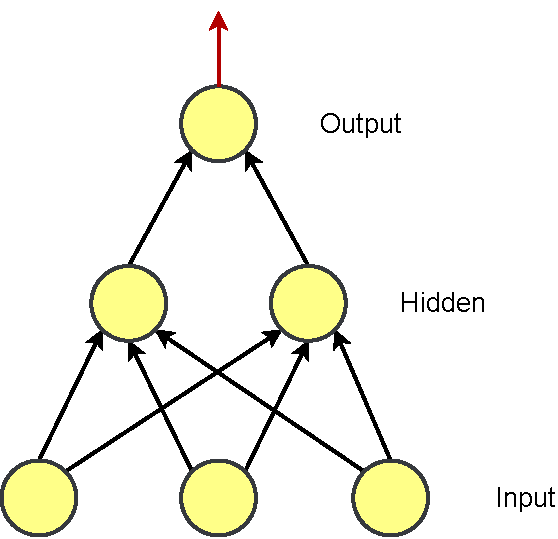
\includegraphics[height=0.7\textheight]{./mlnn_out}
\end{center}
}

%\frame{
%\frametitle{Multilayer Neural Network}
%\begin{center}
%\includegraphics[width=\linewidth]{./ml1}
%\end{center}
%}

\frame{
	\frametitle{Output}
Output layer ($k$):
\begin{equation}
o_k = f \left( \sum_j w_{jk} a_j + b_k \right) 
\end{equation}
\begin{center}
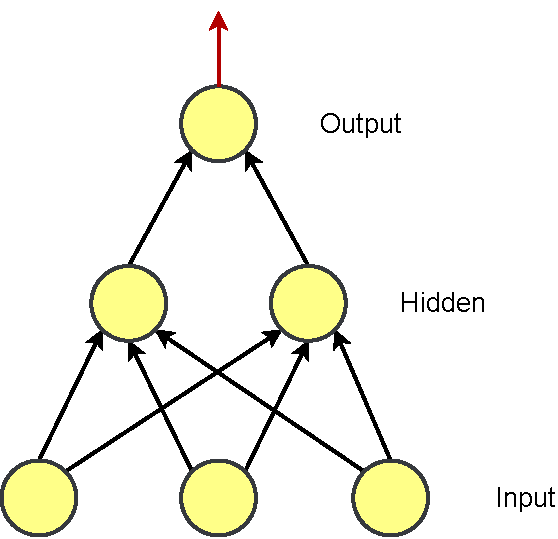
\includegraphics[height=0.5\textheight]{./mlnn_out}
\end{center}
}


\frame{
	\frametitle{Weights}
	\begin{itemize}
		\item Now the weights are labeled $w_{i,j}$, where $i$ denotes input unit and $j$ denotes the hidden node
	\begin{center}
	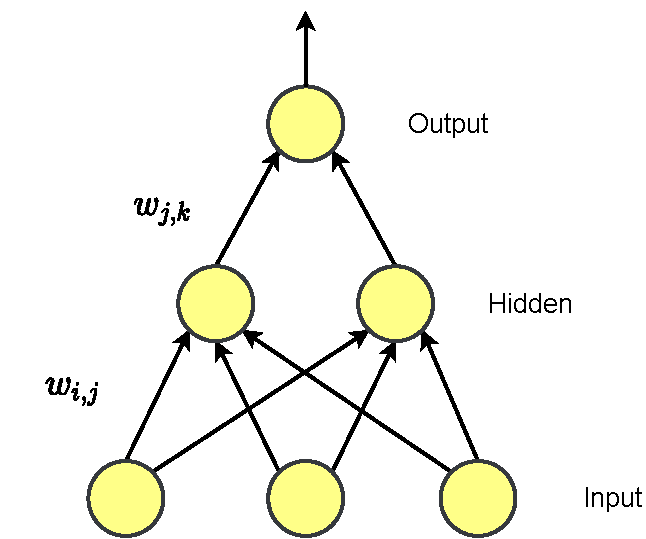
\includegraphics[height=0.7\textheight]{./mlnn_we}
	\end{center}
	\end{itemize}
}	


%\frame{
%	\frametitle{Weights}
%	\begin{itemize}
%		\item Example
%		
%\begin{center}
%\includegraphics[width=0.8\linewidth]{./network-with-labeled-weights}
%\end{center}
%	\end{itemize}
%}


\frame{
	\frametitle{Weights (2)}
	\begin{itemize}
		\item The weights are stored in matrices
\begin{center}
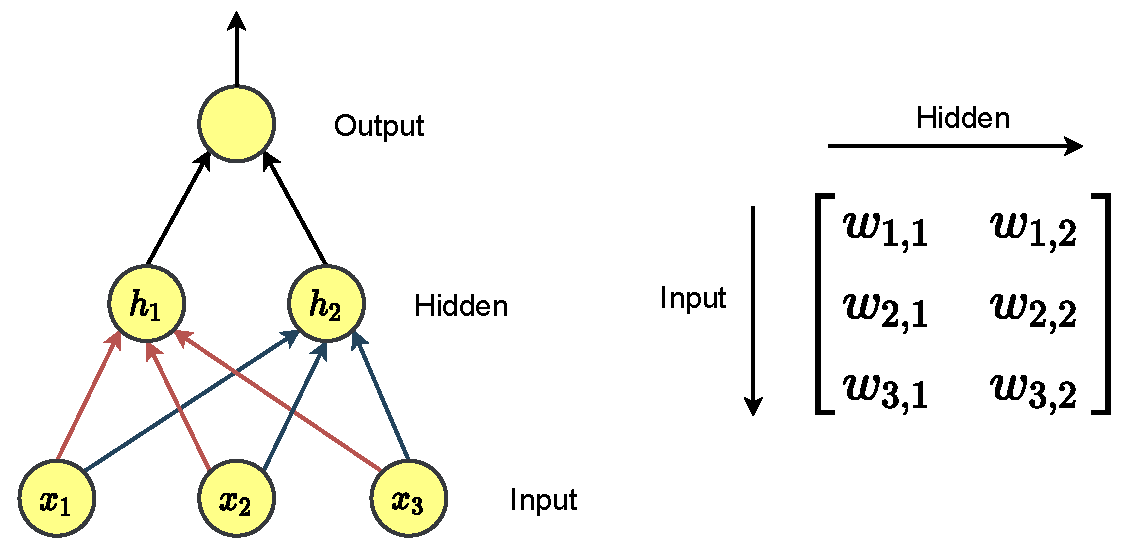
\includegraphics[height=0.55\textheight]{./mlnn_weights}
\end{center}
	\end{itemize}
}


\frame{
	\frametitle{Weights (3)}
	\begin{itemize}
		\item The weights are stored in matrices
		\begin{center}
			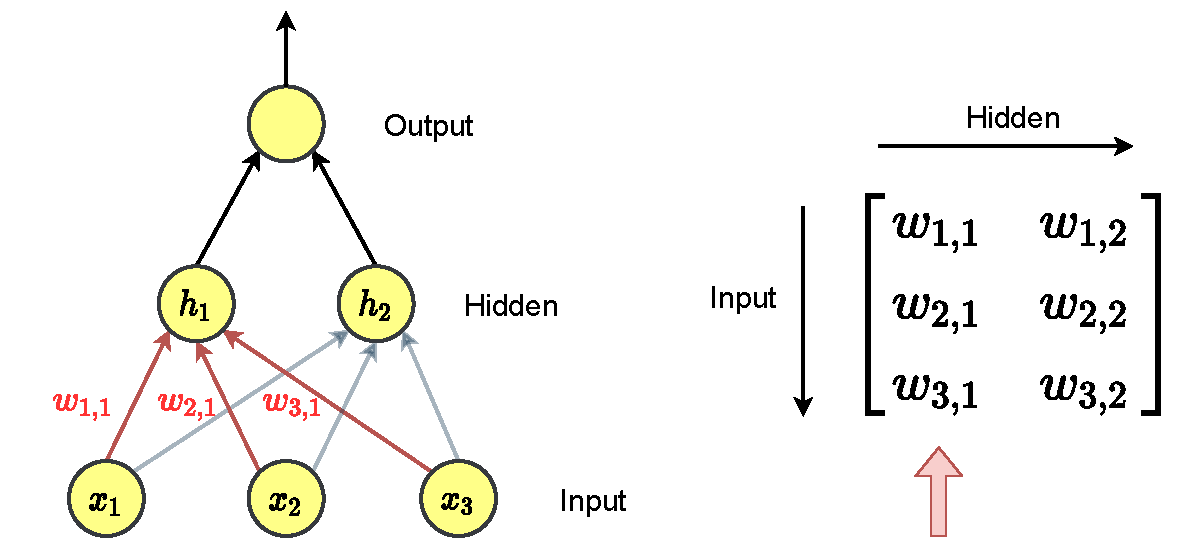
\includegraphics[height=0.55\textheight]{./mlnn_wl}
		\end{center}
	\end{itemize}
}



\frame{
	\frametitle{Weights (4)}
	\begin{itemize}
		\item The weights are stored in matrices
		\begin{center}
			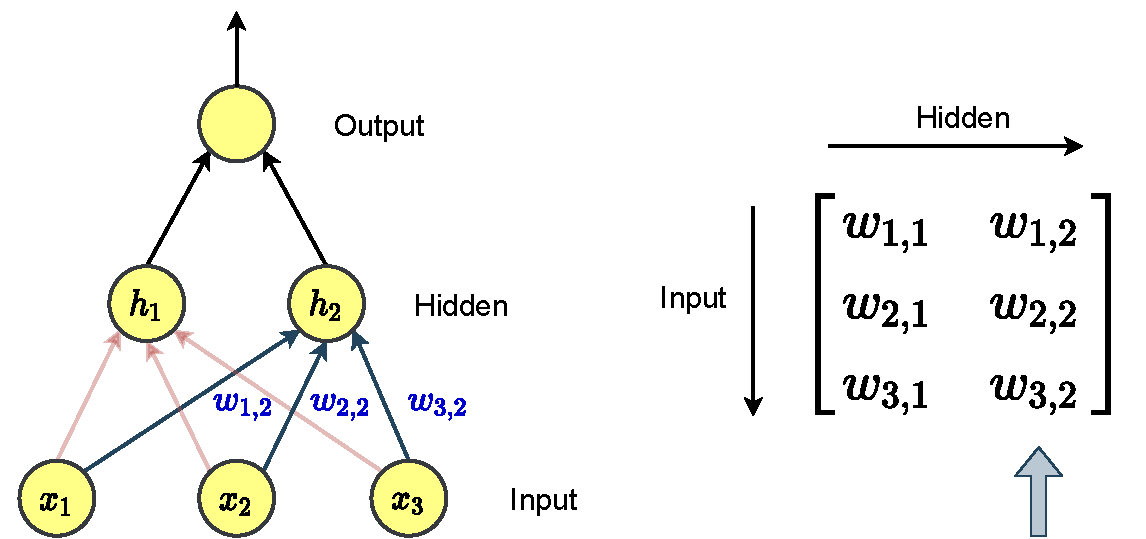
\includegraphics[height=0.55\textheight]{./mlnn_wr}
		\end{center}
	\end{itemize}
}


\begin{frame}
	\frametitle{Hidden Layers}
	Each $i$-th layer is composed of:
	\begin{itemize}
		\item The weights, $$W_i = \begin{bmatrix}
			w_{1,1} & \dots & w_{1,n}
			\\
			\vdots & \ddots & \vdots
			\\
			w_{m,1} & \dots & w_{m,n}
			\\
		\end{bmatrix}$$, where $m$ is the amount of inputs and $n$ the outputs
		\item The bias, $$ B_i = [b_1, \dots, b_n] $$
		\item The activation function can be different for each layer, $f_i(H)$
	\end{itemize}
\end{frame}


\section{Inference}

\frame{
\frametitle{Inference}
\begin{itemize}
%\item  Input to hidden node j 
%\begin{equation}
%	h_j = \sum_i w_{i,j} x_i + b_j
%\end{equation}
\item From now on, we will use matrices
\begin{equation}
	H_i = A_{i-1}W_i + B_i
\end{equation}
e.g.
$$
	H_1 =  \begin{bmatrix}
	x_{1} & x_{2} & x_3
	\end{bmatrix} 
	\begin{bmatrix}
	w_{1,1} & w_{1,2}
	\\
	w_{2,1} & w_{2,2}
	\\
	w_{3,1} & w_{3,2}
	\\
	\end{bmatrix} + \begin{bmatrix}
b_{1} & b_{2} 
\end{bmatrix} 
$$
\item $H_i$ is introduced to the activation function, then
\begin{equation}
	A_i = f_i (H_i)
\end{equation}
\item if $i$ is the last layer, then
\begin{equation}
\hat{Y} = H_i	
\end{equation}
$$\hat{Y} = f([h_1, h_2])$$
\end{itemize}
}




\frame{
	\frametitle{Parameters}
	\begin{itemize}
		\item Inference
		\begin{equation}
			X \rightarrow f(XW_1 + B_1) \rightarrow A_1 \rightarrow f_2(A_1W_2 + B_2) \rightarrow \hat{Y} 
		\end{equation}
		
		\begin{figure}
			\centering
			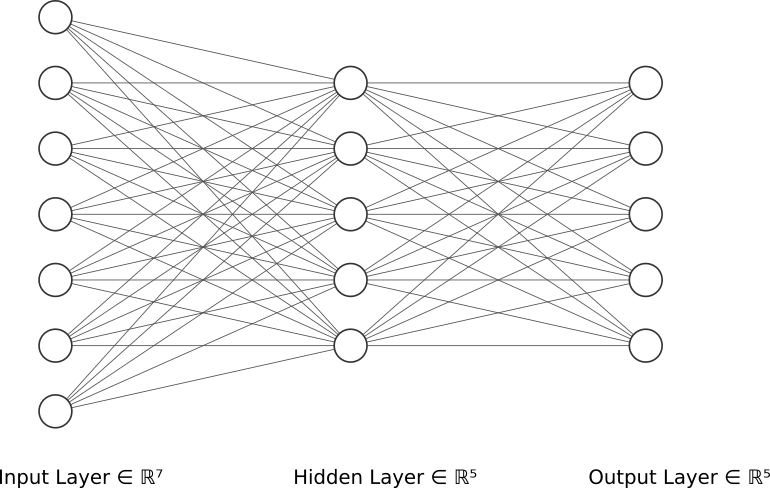
\includegraphics[height=0.5\textheight]{nn_simple1}
			%\caption{Example of a NN}
			\label{fig:nnsimple1}
		\end{figure}
		\item Number of parameters in each layer:
		\begin{equation}
			c(m,n) = (m + 1) n
		\end{equation} where $m$ is the number of inputs and $n$ the number of outputs.
	\end{itemize}
}


\begin{frame}
	\frametitle{Exercise}
	Tomando en cuenta la siguiente red neuronal multicapa: 
	\begin{columns}
		\begin{column}{0.3\textwidth}
			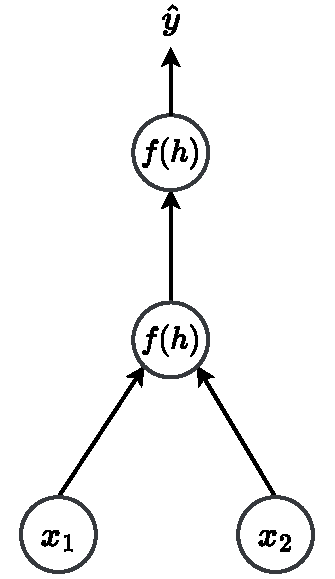
\includegraphics[height=0.5\textheight]{mlnn_example_211.pdf}
		\end{column}
		\begin{column}{0.5\textwidth}  %%<--- here
			\begin{center}
				\begin{itemize}
					\item Input:
					$$X = [ 0.1, 0.2 ]$$
					\item Layer 1:
					$$ W_1 = \begin{bmatrix} 
						-0.5 \\
						0.4
					\end{bmatrix}, B_1 = [0], f_1(H) = sigmoid()
					$$
					\item Layer 2:
					$$
						W_2 = \begin{bmatrix}
						0.3
					\end{bmatrix}, B_2 = [1], f_2(H) = tanh()
					$$
				\end{itemize}
			\end{center}
		\end{column}
	\end{columns}
	\begin{enumerate}
	\item Calcule la salida de la capa oculta (Utilice notación matricial). 
	\item Calcule la predicción de la red. 
	\end{enumerate}  
\end{frame}


\frame{
	\frametitle{Excercises}
	\begin{itemize}
		\item Determine the amount of weights required in the following network:
		
		\begin{figure}
			\centering
			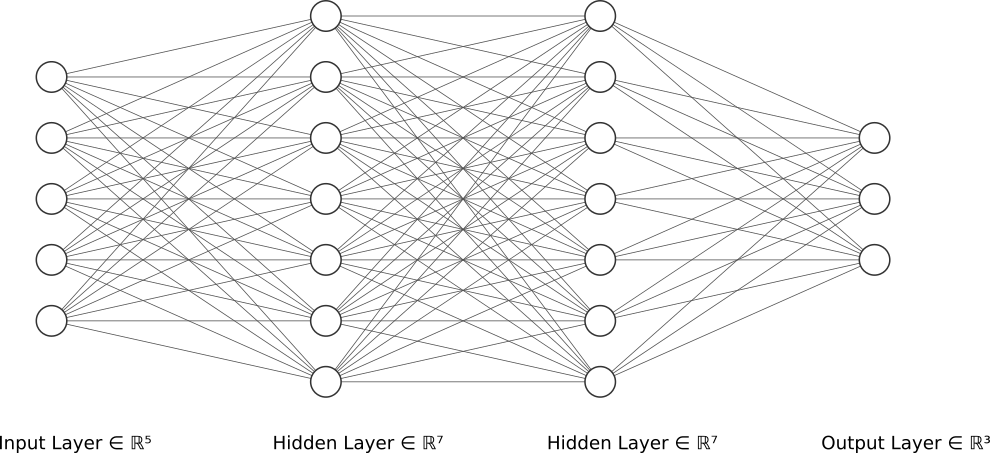
\includegraphics[height=0.6\textheight]{nn}
			%	\caption{}
			\label{fig:nn}
		\end{figure}
	\end{itemize}
}



\begin{frame}
	\frametitle{Multilayer network predictions}
	\begin{columns}
		\begin{column}{0.5\textwidth}
			
\includegraphics[width=0.9\textwidth]{./friend}
		\end{column}
		\begin{column}{0.5\textwidth}  %%<--- here
			\begin{center}
				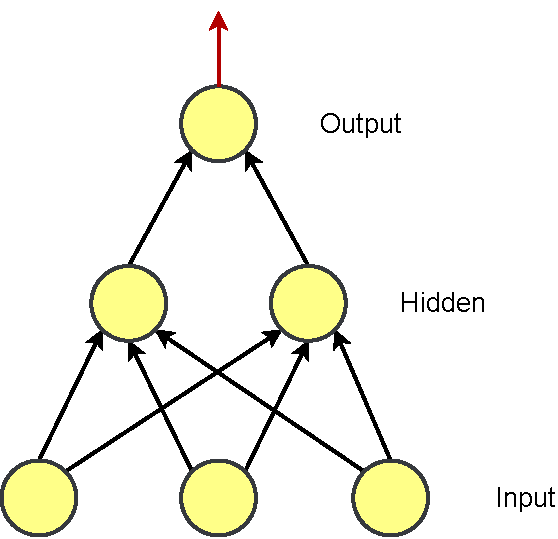
\includegraphics[width=0.7\textwidth]{./mlnn_out}
			\end{center}
		\end{column}
	\end{columns}
\end{frame}


\section{Backpropagation}


\frame{
\frametitle{Backpropagation\footnote{Rumelhart, D. E., Hinton, G. E., \& Williams, R. J. (1986). Learning representations by back-propagating errors. nature, 323(6088), 533-536.}}
\begin{itemize}
\item How do we find the errors for the gradient descent step?
\begin{center}
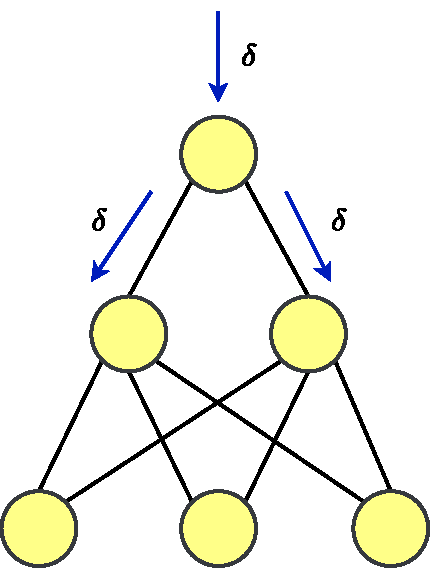
\includegraphics[height=0.6\textheight]{backprop_intro.drawio.pdf}
\end{center}
\end{itemize}
}


\frame{
\frametitle{Backpropagation introduction}
	\begin{itemize}
	\item The errors are proportional to the error in the output layer times the weight between the units.
\begin{center}
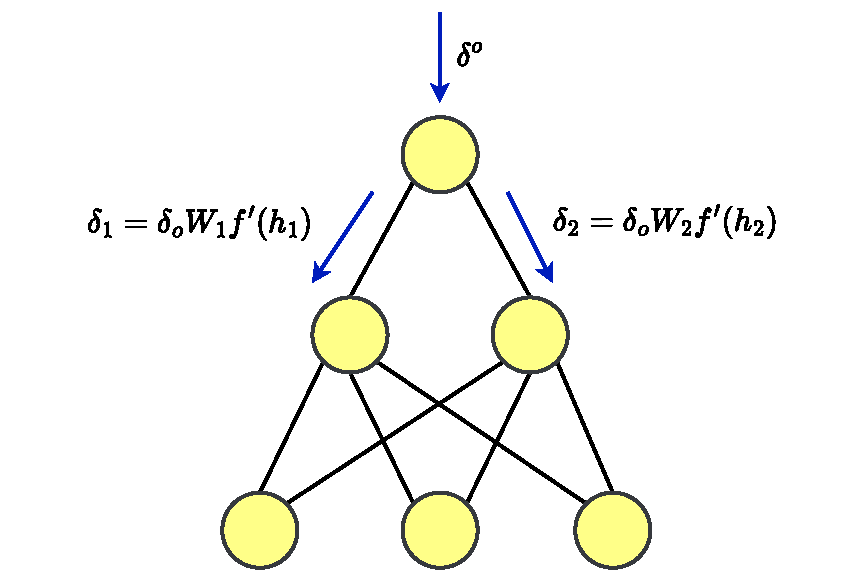
\includegraphics[height=0.6\textheight]{./backprop_deltas}
\end{center}
	\end{itemize}
}


\frame{
\frametitle{Ready, set...}
\begin{center}
	
\includegraphics[height=0.6\textheight]{brace}
\end{center}
}


\frame{
	\frametitle{Backpropagation rules}
	\begin{itemize}
		\item It is an extension of the gradient descent
		\item General contribution of the weight:
		\begin{equation}
		\frac{\partial E}{\partial w_{h,o}} = \frac{\partial E}{\partial h_o} \frac{\partial h_o}{\partial w_{h,o}}  =   \frac{\partial E}{\partial h_o} y_h
		\end{equation} where $o$ indicates the output layer and $h$ indicates the hidden layer.
		\item General update rule:
		\begin{equation}
			w^{new} = w^{old} + (-1) \eta \frac{\partial E}{w^{old}}
		\end{equation}

	\end{itemize}
}


\frame{
\frametitle{Backprogation implementation}
\begin{itemize}
\item In the output layer you have errors in each unit $o$,
\item We can generalize previous error term as $\delta_o$,
\item Term error for hidden layer node $h$,
\begin{equation}
	\delta_h = \sum_o w_{h,o} \delta_o f'(h_h)
\end{equation}

\item The gradient descent step is the same, $$\Delta w_{i,h} = \eta \delta_h x_{h}$$
\end{itemize}
}


%\frame{
%\frametitle{Example}
%\begin{center}
%\includegraphics[height=0.8\textheight]{./backprop-network}
%\end{center}
%}


\frame{
\frametitle{Backprogation Algorithm}
Initialization
\begin{itemize}
\item Set the weight steps for each layer to zero
\begin{itemize}
	\item The input to hidden weights $\Delta w_{h,o} = 0$
	\item The hidden to output eights $\Delta W_{i,h} = 0$
\end{itemize}
\end{itemize}
}


\frame{
\frametitle{Backpropagation algorithm (special case)}

While we are doing gradient descent for a given number of epochs.

\begin{enumerate}
\item For each $x \in Data$ 
	\begin{enumerate}
		\item Make a forward pass, $\hat{y} = f(xW)$
		\item Calculate the error term in the output unit $\delta_o = (y-\hat{y})f'(h)$
		\item Propagate the errors to hidden layer $\delta_h = \delta_o W_h f'(h_h)$
		\item Update the weight steps: \\ 
		$\Delta w_{h,o} = \Delta w_{h,o} + \delta_o \hat{y}_h$ \\
		$\Delta w_{i,h} = \Delta w_{i,h} + \delta_h x_i$
	\end{enumerate}
\item Update the weights, where $\eta$ is the learning rate and $m$ is the number of records: \\ 
$w_{h,o} = w_{h,o} + \frac{\eta}{m} \Delta w_{h,o}$ \\ 
$w_{i,h} = w_{i,h} + \frac{\eta}{m} \Delta w_{i,h}$
\end{enumerate}
}


\begin{frame}
	\frametitle{Award}
	
	\begin{figure}
		\centering
		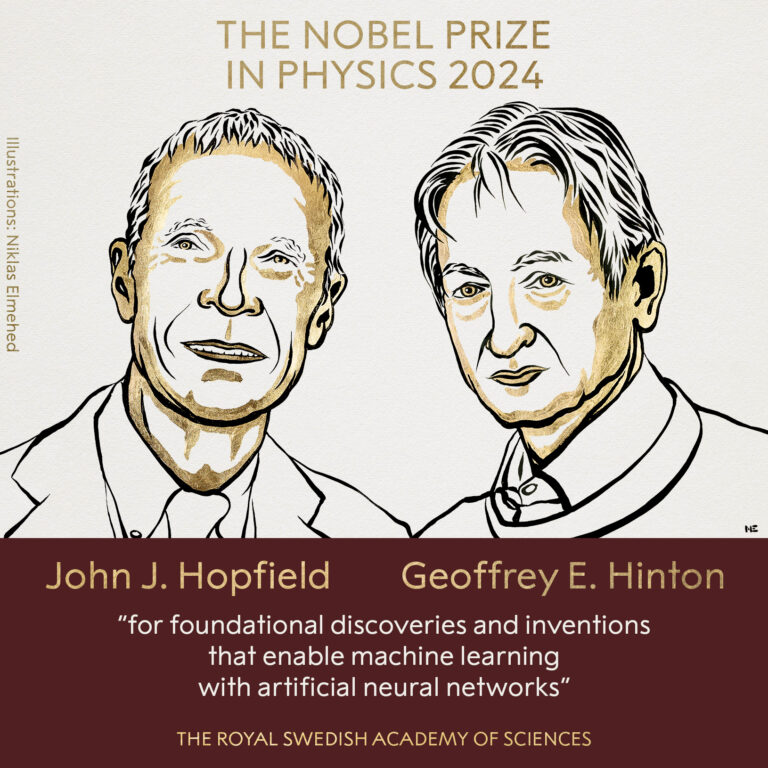
\includegraphics[height=0.8\textheight]{fisica-768x768}
		%\caption{}
		%\label{fig:fisica-768x768}
	\end{figure}
\end{frame}


\frame{
\frametitle{Backpropagation remarks}

\begin{itemize}
	\item Backpropagation is fundamental in neural networks.
	\item It is already implemented in many frameworks.
	\item As engineers/scientists we have to understand it very well.
\end{itemize}

\pause

\begin{center}
	
\includegraphics[height=0.5\textheight]{robin}
\end{center}
}




%\frame{
%\frametitle{Extra Resources}
%Linear algebra
%\begin{itemize}
%\item Khan academy introduction to vectors. 
%\item Khan academy introduction to matrices
%\end{itemize}
%Backpropagation is fundamental to deep learning. TensorFlow and other libraries will perform the backprop for you, but you should really really understand the algorithm. 
%\begin{itemize}
%\item \url{https://medium.com/@karpathy/yes-you-should-understand-backprop-e2f06eab496b}
%\item \url{https://youtu.be/59Hbtz7XgjM}
% \end{itemize}
%}



%\frame{
%\frametitle{Exercise}
%\begin{itemize}
%\item Implement the backpropagation algorithm for a network trained on the graduate school admission data
%\item Implement the forward pass
%\item Implement the backpropagation
%\item Update the weights
%\end{itemize}
%}

\frame{
\frametitle{Further readings}
\begin{itemize}
	\item IEEE Spectrum (2024) 'Nobel Prize in Physics for Machine Learning Pioneers', IEEE Spectrum, 8 de octubre. Disponible en:  \url{https://spectrum.ieee.org/nobel-prize-in-physics} (Accedido: 4 de febrero de 2026).
\end{itemize}
}

\frame{
\frametitle{References}
\begin{itemize}
\item \textbf{Section 6.5, Back propagation and other diferentiation algorithms.} Goodfellow, Ian, et al. Deep learning. Vol. 1. No. 2. Cambridge: MIT press, 2016.
\item \textbf{The back propagation algorithm.} Buduma, N., Buduma, N., \& Papa, J. (2022). Fundamentals of deep learning. " O'Reilly Media, Inc.".
\item \textbf{4.6 Backpropagation.} Skansi, S. (2018). Introduction to Deep Learning: from logical calculus to artificial intelligence. Springer.
\item Stewart, James, Daniel K. Clegg, and Saleem Watson. Calculus: early transcendentals. Cengage Learning, 2020.
%\item Udacity - Self Driving Car Nanodegree
\end{itemize}
}


\begin{frame}
\frametitle{Where we are in the history?}
\begin{figure}
	\centering
	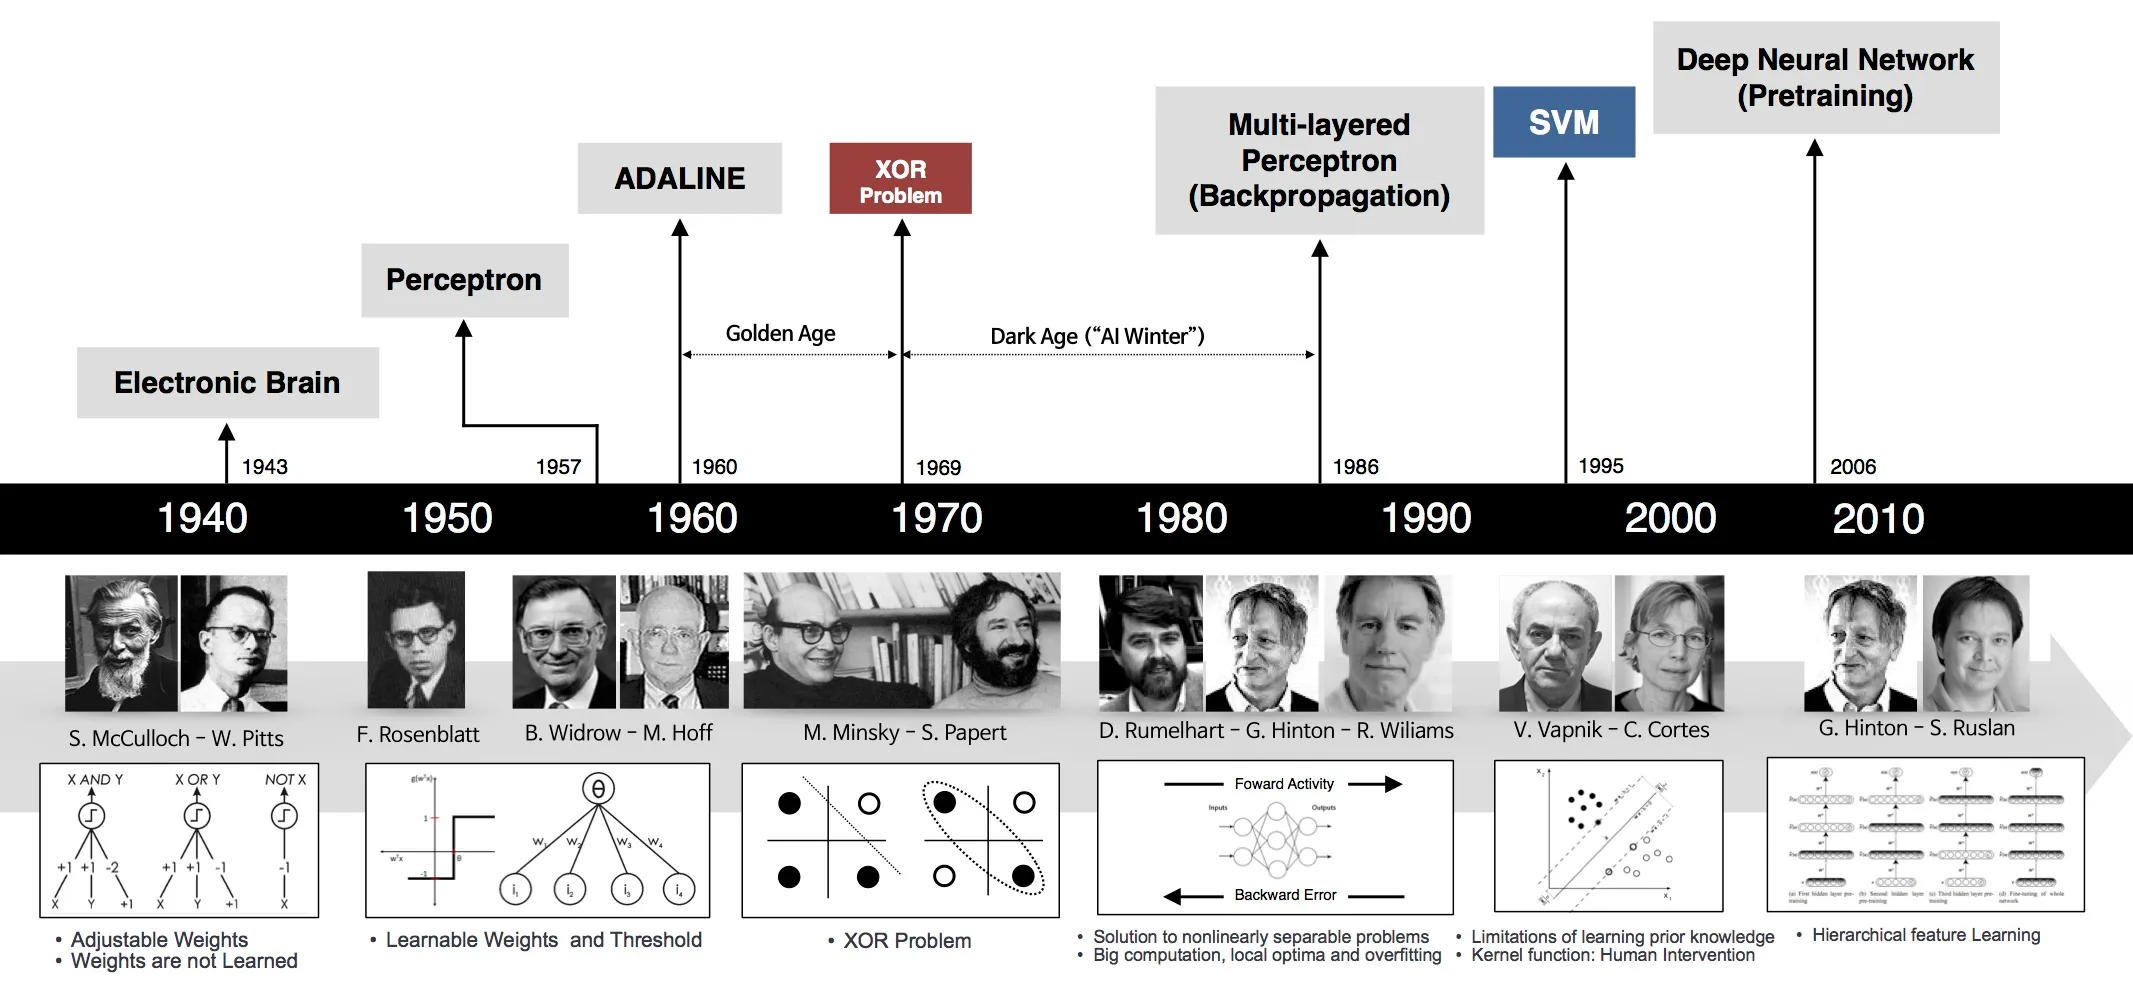
\includegraphics[height=0.7\textheight]{nn_timeline}
	\caption{Brieft history of the neural networks \footnote{\tiny Sefik Ilkin Serengil, Evolution of Neural Networks, sefiks.com, Consulted: october 2024}.}
	\label{fig:nntimeline}
\end{figure}
\end{frame}



\end{document}